\documentclass{article}\usepackage[]{graphicx}\usepackage[]{xcolor}
% maxwidth is the original width if it is less than linewidth
% otherwise use linewidth (to make sure the graphics do not exceed the margin)
\makeatletter
\def\maxwidth{ %
  \ifdim\Gin@nat@width>\linewidth
    \linewidth
  \else
    \Gin@nat@width
  \fi
}
\makeatother

\definecolor{fgcolor}{rgb}{0.345, 0.345, 0.345}
\newcommand{\hlnum}[1]{\textcolor[rgb]{0.686,0.059,0.569}{#1}}%
\newcommand{\hlsng}[1]{\textcolor[rgb]{0.192,0.494,0.8}{#1}}%
\newcommand{\hlcom}[1]{\textcolor[rgb]{0.678,0.584,0.686}{\textit{#1}}}%
\newcommand{\hlopt}[1]{\textcolor[rgb]{0,0,0}{#1}}%
\newcommand{\hldef}[1]{\textcolor[rgb]{0.345,0.345,0.345}{#1}}%
\newcommand{\hlkwa}[1]{\textcolor[rgb]{0.161,0.373,0.58}{\textbf{#1}}}%
\newcommand{\hlkwb}[1]{\textcolor[rgb]{0.69,0.353,0.396}{#1}}%
\newcommand{\hlkwc}[1]{\textcolor[rgb]{0.333,0.667,0.333}{#1}}%
\newcommand{\hlkwd}[1]{\textcolor[rgb]{0.737,0.353,0.396}{\textbf{#1}}}%
\let\hlipl\hlkwb

\usepackage{framed}
\makeatletter
\newenvironment{kframe}{%
 \def\at@end@of@kframe{}%
 \ifinner\ifhmode%
  \def\at@end@of@kframe{\end{minipage}}%
  \begin{minipage}{\columnwidth}%
 \fi\fi%
 \def\FrameCommand##1{\hskip\@totalleftmargin \hskip-\fboxsep
 \colorbox{shadecolor}{##1}\hskip-\fboxsep
     % There is no \\@totalrightmargin, so:
     \hskip-\linewidth \hskip-\@totalleftmargin \hskip\columnwidth}%
 \MakeFramed {\advance\hsize-\width
   \@totalleftmargin\z@ \linewidth\hsize
   \@setminipage}}%
 {\par\unskip\endMakeFramed%
 \at@end@of@kframe}
\makeatother

\definecolor{shadecolor}{rgb}{.97, .97, .97}
\definecolor{messagecolor}{rgb}{0, 0, 0}
\definecolor{warningcolor}{rgb}{1, 0, 1}
\definecolor{errorcolor}{rgb}{1, 0, 0}
\newenvironment{knitrout}{}{} % an empty environment to be redefined in TeX

\usepackage{alltt}
\usepackage[margin=1.0in]{geometry} % To set margins
\usepackage{amsmath}  % This allows me to use the align functionality.
                      % If you find yourself trying to replicate
                      % something you found online, ensure you're
                      % loading the necessary packages!
\usepackage{amsfonts} % Math font
\usepackage{fancyvrb}
\usepackage{hyperref} % For including hyperlinks
\usepackage[shortlabels]{enumitem}% For enumerated lists with labels specified
                                  % We had to run tlmgr_install("enumitem") in R
\usepackage{float}    % For telling R where to put a table/figure
\usepackage{natbib}        %For the bibliography
\bibliographystyle{apalike}%For the bibliography
\IfFileExists{upquote.sty}{\usepackage{upquote}}{}
\begin{document}


\begin{enumerate}
%%%%%%%%%%%%%%%%%%%%%%%%%%%%%%%%%%%%%%%%%%%%%%%%%%%%%%%%%%%%%%%%%%%%%%%%%%%%%%%%
%%%%%%%%%%%%%%%%%%%%%%%%%%%%%%%%%%%%%%%%%%%%%%%%%%%%%%%%%%%%%%%%%%%%%%%%%%%%%%%%
% Question 1
%%%%%%%%%%%%%%%%%%%%%%%%%%%%%%%%%%%%%%%%%%%%%%%%%%%%%%%%%%%%%%%%%%%%%%%%%%%%%%%%
%%%%%%%%%%%%%%%%%%%%%%%%%%%%%%%%%%%%%%%%%%%%%%%%%%%%%%%%%%%%%%%%%%%%%%%%%%%%%%%%
\item When conducting the work of Lab 11, we conducted the test that uses the
Central Limit Theorem even though the sample size was ``small" (i.e., $n<30$).
It turns out, that how ``far off" the $t$-test is can be computed using
a first-order Edgeworth approximation for the error. Below, we will do this 
for the the further observations.
\begin{enumerate}
  \item \cite{Boos00} note that 
  \begin{align*}
    P(T \leq t) \approx F_Z(t) + \underbrace{\frac{\text{skew}}{\sqrt{n}} \frac{(2t^2+1)}{6} f_Z(t)}_{\textrm{error}},
  \end{align*}
  where $f_Z(\cdot)$ and $F_Z(\cdot)$ are the Gaussian PDF and CDF and skew is the
  skewness of the data. What is the potential error in the computation of the 
  $p$-value when testing $H_0: \mu_X=0; H_a: \mu_X<0$ using the zebra finch further data? 
\begin{knitrout}\scriptsize
\definecolor{shadecolor}{rgb}{0.969, 0.969, 0.969}\color{fgcolor}\begin{kframe}
\begin{alltt}
\hlcom{#read the data file}
\hldef{dat.finches} \hlkwb{<-} \hlkwd{read_csv}\hldef{(}\hlsng{"zebrafinches.csv"}\hldef{)}
\hlcom{#separate further column}
\hldef{dat.further} \hlkwb{<-} \hldef{dat.finches}\hlopt{$}\hldef{further}

\hldef{mu0} \hlkwb{=} \hlnum{0}
\hlcom{#compute t-statistics to get the t-value for the further data}
\hldef{t_furth} \hlkwb{<-} \hlkwd{t.test}\hldef{(dat.further,} \hlkwc{mu} \hldef{= mu0,} \hlkwc{alternative} \hldef{=} \hlsng{"less"}\hldef{)}
\hldef{t} \hlkwb{<-} \hldef{t_furth}\hlopt{$}\hldef{statistic} \hlcom{#extract t}
\hldef{n} \hlkwb{<-} \hlkwd{length}\hldef{(dat.further)} \hlcom{#get n}

\hlcom{#calculate skewness of data}
\hldef{skew} \hlkwb{<-} \hlkwd{skewness}\hldef{(dat.further)}

\hlcom{#use Gaussian pdf and calculate the error}
\hldef{pdf.finches} \hlkwb{<-} \hlkwd{dnorm}\hldef{(t,} \hlkwc{mean} \hldef{=} \hlnum{0}\hldef{,} \hlkwc{sd} \hldef{=} \hlnum{1}\hldef{)}
\hldef{potential.error} \hlkwb{<-} \hldef{(skew}\hlopt{/}\hlkwd{sqrt}\hldef{(n))}\hlopt{*}\hldef{((}\hlnum{2}\hlopt{*}\hldef{t}\hlopt{^}\hlnum{2} \hlopt{+}\hlnum{1}\hldef{)}\hlopt{/}\hlnum{6}\hldef{)}\hlopt{*}\hldef{pdf.finches}

\hldef{potential.error}
\end{alltt}
\begin{verbatim}
##             t 
## -1.226006e-13
\end{verbatim}
\end{kframe}
\end{knitrout}
The potential error in the computation of the $p$-value when testing $H_0: \mu_X=0; H_a: \mu_X<0$ using the zebra finch further data is \ensuremath{-1.2260063\times 10^{-13}}, which is extremely close to 0. Therefore, the t-test results on the zebra finch further data can be trusted even though the sample size is small. The Central Limit Theorem approximation works very well for the data. The error is negative, which means the true $p$-value is slightly lower than we assumed.
  \item Compute the error for $t$ statistics from -10 to 10 and plot a line
  that shows the error across $t$. Continue to use the skewness and 
  the sample size for the zebra finch further data.
  
\begin{knitrout}\scriptsize
\definecolor{shadecolor}{rgb}{0.969, 0.969, 0.969}\color{fgcolor}\begin{kframe}
\begin{alltt}
\hlcom{#generate a vector of t-values and compute pdf for each of them}
\hldef{t.vals} \hlkwb{<-} \hlkwd{seq}\hldef{(}\hlkwc{from} \hldef{=} \hlopt{-}\hlnum{10}\hldef{,} \hlkwc{to} \hldef{=} \hlnum{10}\hldef{,} \hlkwc{length.out} \hldef{=} \hlnum{1000}\hldef{)}
\hldef{pdf.t.vals} \hlkwb{<-} \hlkwd{dnorm}\hldef{(t.vals,} \hlkwc{mean} \hldef{=} \hlnum{0}\hldef{,} \hlkwc{sd} \hldef{=} \hlnum{1}\hldef{)}

\hlcom{#calculate the error across of all t}
\hldef{t.potential.error} \hlkwb{<-} \hldef{(skew}\hlopt{/}\hlkwd{sqrt}\hldef{(n))}\hlopt{*}\hldef{((}\hlnum{2}\hlopt{*}\hldef{t.vals}\hlopt{^}\hlnum{2} \hlopt{+}\hlnum{1}\hldef{)}\hlopt{/}\hlnum{6}\hldef{)}\hlopt{*}\hldef{pdf.t.vals}

\hlcom{#create a tibble to plot the errors for t-statistics}
\hldef{dat.error.plot} \hlkwb{<-} \hlkwd{tibble}\hldef{(t.vals, t.potential.error)}

\hlcom{#plot the error for the t-statistics }
\hldef{error.plot} \hlkwb{<-} \hlkwd{ggplot}\hldef{(dat.error.plot)}\hlopt{+}
\hlkwd{geom_line}\hldef{(}\hlkwd{aes}\hldef{(}\hlkwc{x}\hldef{= t.vals,} \hlkwc{y} \hldef{= t.potential.error))}\hlopt{+} \hlcom{#plot the line for the errors}
\hlkwd{theme_bw}\hldef{()}\hlopt{+}
\hlkwd{labs}\hldef{(}\hlkwc{title} \hldef{=} \hlsng{"Edgeworth approximation for the error for p-value"}\hldef{,}
     \hlkwc{x} \hldef{=} \hlsng{"t-statistics"}\hldef{,}
     \hlkwc{y} \hldef{=} \hlsng{"Potential error"}\hldef{)}
\end{alltt}
\end{kframe}
\end{knitrout}
\begin{figure}[H] \begin{center}
\begin{knitrout}
\definecolor{shadecolor}{rgb}{0.969, 0.969, 0.969}\color{fgcolor}
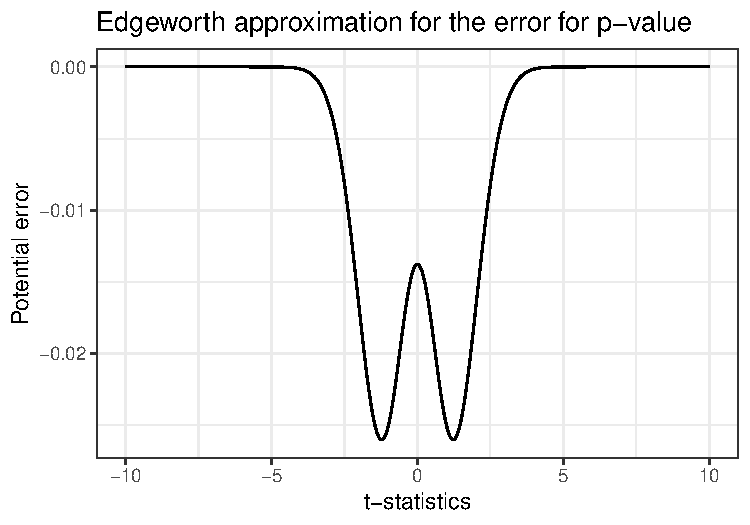
\includegraphics[width=\maxwidth]{figure/unnamed-chunk-4-1} 
\end{knitrout}
\caption{Edgeworth approximation for the error for p-value across t} \label{plot.error} 
\end{center}
\end{figure}


The potential error in $p$-value estimation is minimal across all $t$ values, which supports the validity of t-test approximation. As $t$ gets closer to -10 and 10, the potential error is close to 0. The error becomes larger as $t$ approaches 0. However, when $t$ is very close to 0, the error decreases.

  \item Suppose we wanted to have a tail probability within 10\% of the desired
  $\alpha=0.05$. Recall we did a left-tailed test using the further data.
  How large of a sample size would we need? That is, we need
  to solve the error formula equal to 10\% of the desired left-tail probability:
  \[0.10 \alpha  \stackrel{set}{=} \underbrace{\frac{\text{skew}}{\sqrt{n}} \frac{(2t^2+1)}{6} f_Z(t)}_{\textrm{error}},\]
  which yields
  \[ n = \left(\frac{\text{skew}}{6(0.10\alpha)} (2t^2 + 1) f_Z(t)\right)^2.\]
\begin{knitrout}\scriptsize
\definecolor{shadecolor}{rgb}{0.969, 0.969, 0.969}\color{fgcolor}\begin{kframe}
\begin{alltt}
\hldef{alpha} \hlkwb{<-} \hlnum{0.05}
\hlcom{#calculate the critical value for the left-tailed test}
\hldef{t.crit} \hlkwb{<-} \hlkwd{qnorm}\hldef{(alpha,} \hlkwc{mean} \hldef{=} \hlnum{0}\hldef{,} \hlkwc{sd} \hldef{=} \hlnum{1}\hldef{)}

\hlcom{#calculate pdf}
\hldef{pdf.sample} \hlkwb{<-} \hlkwd{dnorm}\hldef{(t.crit,} \hlkwc{mean} \hldef{=} \hlnum{0}\hldef{,} \hlkwc{sd} \hldef{=} \hlnum{1}\hldef{)}

\hlcom{#calculate n }
\hldef{n.sample} \hlkwb{<-} \hldef{(skew}\hlopt{/}\hldef{(}\hlnum{6}\hlopt{*}\hldef{(}\hlnum{0.10}\hlopt{*}\hldef{alpha))}\hlopt{*}\hldef{(}\hlnum{2}\hlopt{*}\hldef{t.crit}\hlopt{^}\hlnum{2}\hlopt{+}\hlnum{1}\hldef{)}\hlopt{*}\hldef{pdf.sample)}\hlopt{^}\hlnum{2}
\hldef{n.sample} \hlkwb{<-} \hlkwd{ceiling}\hldef{(n.sample)} \hlcom{#round n to the closest positive integer}
\hldef{n.sample}
\end{alltt}
\begin{verbatim}
## [1] 521
\end{verbatim}
\end{kframe}
\end{knitrout}
We would need a sample size of $n = $ 521 to have a tail probability within 10\% of the desired
  $\alpha=0.05$. This large sample size compensates for the skewness in the data, controlling the approximation error.
\end{enumerate}
%%%%%%%%%%%%%%%%%%%%%%%%%%%%%%%%%%%%%%%%%%%%%%%%%%%%%%%%%%%%%%%%%%%%%%%%%%%%%%%%
%%%%%%%%%%%%%%%%%%%%%%%%%%%%%%%%%%%%%%%%%%%%%%%%%%%%%%%%%%%%%%%%%%%%%%%%%%%%%%%%
% Question 2
%%%%%%%%%%%%%%%%%%%%%%%%%%%%%%%%%%%%%%%%%%%%%%%%%%%%%%%%%%%%%%%%%%%%%%%%%%%%%%%%
%%%%%%%%%%%%%%%%%%%%%%%%%%%%%%%%%%%%%%%%%%%%%%%%%%%%%%%%%%%%%%%%%%%%%%%%%%%%%%%%
\item Complete the following steps to revisit the analyses from lab 11 using the
bootstrap procedure.
\begin{enumerate}
\item Now, consider the zebra finch data. We do not know the generating distributions
for the closer, further, and difference data, so perform resampling to approximate the 
sampling distribution of the $T$ statistic:
  \[T = \frac{\bar{x}_r - 0}{s/\sqrt{n}},\]
  where $\bar{x}_r$ is the mean computed on the r$^{th}$ resample and $s$ is the
  sample standard deviation from the original samples. At the end, create an
  object called \texttt{resamples.null.closer}, for example, and store the 
  resamples shifted to ensure they are consistent with the null hypotheses at the average 
  (i.e., here ensure the shifted resamples are 0 on average, corresponding
  to $t=0$, for each case). 
\begin{knitrout}\scriptsize
\definecolor{shadecolor}{rgb}{0.969, 0.969, 0.969}\color{fgcolor}\begin{kframe}
\begin{alltt}
\hldef{n.resamples} \hlkwb{<-} \hlnum{10000}
\hldef{mu0} \hlkwb{<-} \hlnum{0}

\hlcom{#separate closer and difference data}
\hldef{dat.closer} \hlkwb{<-} \hldef{dat.finches}\hlopt{$}\hldef{closer}
\hldef{dat.diff} \hlkwb{<-} \hldef{dat.finches}\hlopt{$}\hldef{diff}

\hlcom{#get standard deviation}
\hldef{dat.closer.sd} \hlkwb{<-} \hlkwd{sd}\hldef{(dat.closer)}
\hldef{dat.further.sd} \hlkwb{<-} \hlkwd{sd}\hldef{(dat.further)}
\hldef{dat.diff.sd} \hlkwb{<-} \hlkwd{sd}\hldef{(dat.diff)}

\hlcom{#store the approximation of T-statistics}
\hldef{t.stat.storage} \hlkwb{<-} \hlkwd{tibble}\hldef{(}\hlkwc{closer} \hldef{=} \hlkwd{rep}\hldef{(}\hlnum{NA}\hldef{, n.resamples),}
                       \hlkwc{further} \hldef{=} \hlkwd{rep}\hldef{(}\hlnum{NA}\hldef{, n.resamples),}
                       \hlkwc{diff} \hldef{=} \hlkwd{rep}\hldef{(}\hlnum{NA}\hldef{, n.resamples))}

\hlcom{#perform resampling and calculate T-statistics}
\hlkwa{for} \hldef{(i} \hlkwa{in} \hlnum{1}\hlopt{:}\hldef{n.resamples)\{}
\hlcom{#resample}
\hldef{resample.closer} \hlkwb{<-} \hlkwd{sample}\hldef{(dat.closer,} \hlkwc{size} \hldef{= n,} \hlkwc{replace} \hldef{= T)}
\hldef{resample.further} \hlkwb{<-} \hlkwd{sample}\hldef{(dat.further,} \hlkwc{size} \hldef{= n,} \hlkwc{replace} \hldef{= T)}
\hldef{resample.diff} \hlkwb{<-} \hlkwd{sample}\hldef{(dat.diff,} \hlkwc{size} \hldef{= n,} \hlkwc{replace} \hldef{= T)}
\hlcom{#calculate T}
\hldef{t.stat.closer} \hlkwb{<-} \hlkwd{mean}\hldef{(resample.closer)}\hlopt{/}\hldef{(dat.closer.sd}\hlopt{/}\hlkwd{sqrt}\hldef{(n))}
\hldef{t.stat.further} \hlkwb{<-} \hlkwd{mean}\hldef{(resample.further)}\hlopt{/}\hldef{(dat.further.sd}\hlopt{/}\hlkwd{sqrt}\hldef{(n))}
\hldef{t.stat.diff} \hlkwb{<-} \hlkwd{mean}\hldef{(resample.diff)}\hlopt{/}\hldef{(dat.diff.sd}\hlopt{/}\hlkwd{sqrt}\hldef{(n))}
\hlcom{#store the statistics}
\hldef{t.stat.storage}\hlopt{$}\hldef{closer[i]} \hlkwb{=} \hldef{t.stat.closer}
\hldef{t.stat.storage}\hlopt{$}\hldef{further[i]} \hlkwb{=} \hldef{t.stat.further}
\hldef{t.stat.storage}\hlopt{$}\hldef{diff[i]} \hlkwb{=} \hldef{t.stat.diff}
\hldef{\}}

\hlcom{#store the shifted resamples in an object and shift the mean of the data to be 0 under null hypothesis}
\hldef{resamples.null.closer} \hlkwb{<-} \hldef{t.stat.storage}\hlopt{$}\hldef{closer} \hlopt{-} \hlkwd{mean}\hldef{(t.stat.storage}\hlopt{$}\hldef{closer)} \hlopt{+} \hldef{mu0}
\hldef{resamples.null.further} \hlkwb{<-} \hldef{t.stat.storage}\hlopt{$}\hldef{further} \hlopt{-} \hlkwd{mean}\hldef{(t.stat.storage}\hlopt{$}\hldef{further)} \hlopt{+} \hldef{mu0}
\hldef{resamples.null.diff} \hlkwb{<-} \hldef{t.stat.storage}\hlopt{$}\hldef{diff} \hlopt{-} \hlkwd{mean}\hldef{(t.stat.storage}\hlopt{$}\hldef{diff)} \hlopt{+} \hldef{mu0}

\hlcom{#calculate the mean of resamples - should be 0 on average}
\hldef{mean.resample.closer} \hlkwb{<-} \hlkwd{mean}\hldef{(resamples.null.closer)}
\hldef{mean.resample.further} \hlkwb{<-} \hlkwd{mean}\hldef{(resamples.null.further)}
\hldef{mean.resample.diff} \hlkwb{<-} \hlkwd{mean}\hldef{(resamples.null.diff)}

\hldef{mean.resample.closer}
\end{alltt}
\begin{verbatim}
## [1] -5.324852e-16
\end{verbatim}
\begin{alltt}
\hldef{mean.resample.further}
\end{alltt}
\begin{verbatim}
## [1] -1.477152e-16
\end{verbatim}
\begin{alltt}
\hldef{mean.resample.diff}
\end{alltt}
\begin{verbatim}
## [1] 2.280398e-16
\end{verbatim}
\end{kframe}
\end{knitrout}
We performed 10,000 resamples with replacement and computed t-statistics for each resample. Then, we shifted the resamples to make sure that they reflect the null hypothesis. We verified that the shifted resamples were properly centered around 0 by checking that their means were approximately zero: \texttt{mean.resample.closer} = \ensuremath{-5.3248517\times 10^{-16}}, \texttt{mean.resample.further} = \ensuremath{-1.4771517\times 10^{-16}}, and \texttt{mean.resample.diff} = \ensuremath{2.2803981\times 10^{-16}}.
  \item Compute the bootstrap $p$-value for each test using the shifted resamples. 
  How do these compare to the $t$-test $p$-values?
\begin{knitrout}\scriptsize
\definecolor{shadecolor}{rgb}{0.969, 0.969, 0.969}\color{fgcolor}\begin{kframe}
\begin{alltt}
\hlcom{#calculate t-statistics on the original sample}
\hldef{t.obs.closer} \hlkwb{<-} \hlkwd{mean}\hldef{(dat.closer)}\hlopt{/}\hldef{(dat.closer.sd}\hlopt{/}\hlkwd{sqrt}\hldef{(n))}
\hldef{t.obs.further} \hlkwb{<-} \hlkwd{mean}\hldef{(dat.further)}\hlopt{/}\hldef{(dat.further.sd}\hlopt{/}\hlkwd{sqrt}\hldef{(n))}
\hldef{t.obs.diff} \hlkwb{<-} \hlkwd{mean}\hldef{(dat.diff)}\hlopt{/}\hldef{(dat.diff.sd}\hlopt{/}\hlkwd{sqrt}\hldef{(n))}

\hlcom{# p-value: the proportion of observations that are at least as supportive of Ha}
\hldef{p.val.closer} \hlkwb{<-} \hlkwd{mean}\hldef{(resamples.null.closer} \hlopt{>=} \hldef{t.obs.closer)} \hlcom{#right-tailed test}
\hldef{p.val.further} \hlkwb{<-} \hlkwd{mean}\hldef{(resamples.null.further} \hlopt{<=} \hldef{t.obs.further)} \hlcom{#left-tailed test}
\hldef{p.val.diff} \hlkwb{<-} \hlkwd{mean}\hldef{(}\hlkwd{abs}\hldef{(resamples.null.diff)} \hlopt{>=} \hlkwd{abs}\hldef{(t.obs.diff))} \hlcom{#two-tailed test}

\hlcom{#compare with the t-test p-values}
\hldef{t.test.closer} \hlkwb{<-} \hlkwd{t.test}\hldef{(dat.closer,} \hlkwc{mu} \hldef{=} \hlnum{0}\hldef{,} \hlkwc{alternative} \hldef{=} \hlsng{"greater"}\hldef{)}
\hldef{t.test.further} \hlkwb{<-} \hlkwd{t.test}\hldef{(dat.further,} \hlkwc{mu} \hldef{=} \hlnum{0}\hldef{,} \hlkwc{alternative} \hldef{=} \hlsng{"less"}\hldef{)}
\hldef{t.test.diff} \hlkwb{<-} \hlkwd{t.test}\hldef{(dat.diff,} \hlkwc{mu} \hldef{=} \hlnum{0}\hldef{,} \hlkwc{alternative} \hldef{=} \hlsng{"two.sided"}\hldef{)}

\hlcom{#extract their p-values}
\hldef{t.test.closer.p} \hlkwb{<-} \hldef{t.test.closer}\hlopt{$}\hldef{p.value}
\hldef{t.test.further.p} \hlkwb{<-} \hldef{t.test.further}\hlopt{$}\hldef{p.value}
\hldef{t.test.diff.p} \hlkwb{<-} \hldef{t.test.diff}\hlopt{$}\hldef{p.value}

\hlcom{#create a comparison table}
\hldef{comparison.table} \hlkwb{<-}\hlkwd{tibble}\hldef{(}
\hlsng{"Case"} \hldef{=} \hlkwd{c}\hldef{(}\hlsng{"Closer"}\hldef{,} \hlsng{"Further"}\hldef{,} \hlsng{"Difference"}\hldef{),}
\hlsng{"Bootstrap"} \hldef{=} \hlkwd{c}\hldef{(p.val.closer, p.val.further, p.val.diff),}
\hlsng{"T-test"} \hldef{=} \hlkwd{c}\hldef{(t.test.closer.p, t.test.further.p, t.test.diff.p)}
\hldef{)}
\end{alltt}
\end{kframe}
\end{knitrout}
% latex table generated in R 4.4.2 by xtable 1.8-4 package
% Mon Apr 28 21:33:17 2025
\begin{table}[ht]
\centering
\begin{tabular}{lrl}
  \hline
Case & Bootstrap & T-test \\ 
  \hline
Closer & 0.00 & 8.13e-09 \\ 
  Further & 0.00 & 2.59e-08 \\ 
  Difference & 0.00 & 1.04e-08 \\ 
   \hline
\end{tabular}
\caption{Bootstrap and t-test p-values} 
\end{table}

The bootstrap p-values for all three cases were estimated as 0, while the corresponding t-test p-values, although extremely small, were nonzero. The difference arises because the t-test p-values are based on theoretical calculations assuming an approximately normal distribution, which can detect very small probabilities. In contrast, the bootstrapping is based on a finite number of resamples, and with our data it did not produce any extreme t-statistics as the theoretical version. We have statistically discernible evidence against the null hypothesis in each case.

    \item What is the 5$^{th}$ percentile of the shifted resamples under the null hypothesis? 
  Note this value approximates $t_{0.05, n-1}$. Compare these values in each case.
\begin{knitrout}\scriptsize
\definecolor{shadecolor}{rgb}{0.969, 0.969, 0.969}\color{fgcolor}\begin{kframe}
\begin{alltt}
\hlcom{#get 5th percentile of the shifted resamples}
\hldef{close.5th} \hlkwb{<-} \hlkwd{quantile}\hldef{(resamples.null.closer,} \hlkwc{probs} \hldef{=} \hlnum{0.05}\hldef{)}
\hldef{further.5th} \hlkwb{<-} \hlkwd{quantile}\hldef{(resamples.null.further,} \hlkwc{probs} \hldef{=} \hlnum{0.05}\hldef{)}
\hldef{diff.5th} \hlkwb{<-} \hlkwd{quantile}\hldef{(resamples.null.diff,} \hlkwc{probs} \hldef{=} \hlnum{0.05}\hldef{)}

\hlcom{#calculate theoretical t-distribution value}
\hldef{df} \hlkwb{<-} \hldef{n}\hlopt{-}\hlnum{1}
\hlcom{#approximate t0.05,n-1}
\hldef{t.critical.5th} \hlkwb{<-} \hlkwd{qt}\hldef{(}\hlnum{0.05}\hldef{, df)}

\hlcom{#comparison table}
\hldef{comparison.table.percentile} \hlkwb{<-}\hlkwd{tibble}\hldef{(}
\hlsng{"Case"} \hldef{=} \hlkwd{c}\hldef{(}\hlsng{"Closer"}\hldef{,} \hlsng{"Further"}\hldef{,} \hlsng{"Difference"}\hldef{),}
\hlsng{"Bootstrap"} \hldef{=} \hlkwd{c}\hldef{(close.5th, further.5th, diff.5th),}
\hlsng{"Theoretical"} \hldef{=} \hlkwd{rep}\hldef{(t.critical.5th,} \hlnum{3}\hldef{)}
\hldef{)}
\end{alltt}
\end{kframe}
\end{knitrout}
% latex table generated in R 4.4.2 by xtable 1.8-4 package
% Mon Apr 28 21:33:17 2025
\begin{table}[ht]
\centering
\begin{tabular}{lrr}
  \hline
Case & Bootstrap & Theoretical \\ 
  \hline
Closer & -1.61 & -1.71 \\ 
  Further & -1.70 & -1.71 \\ 
  Difference & -1.60 & -1.71 \\ 
   \hline
\end{tabular}
\caption{Bootstrap and theoretical 5th percentile of the shifted resamples under the null hypothesis} 
\end{table}

For the left-tailed hypothesis test, which we use for further data, the critical value for rejecting the null hypothesis is based on the 5th percentile of the shifted resamples. This value approximates $t_{0.05, n-1}$. Our approximation for $t_{0.05, n-1}$ (-1.7) is very close to the theoretical value -1.71. However, the theoretical value is slightly more extreme than the approximation. Therefore, the bootstrapping approximates the t-distribution well. However, we cannot draw concrete conclusions from comparing the right-tailed hypothesis test (closer data) and two-tailed hypothesis test (difference data) to $t_{0.05, n-1}$, as the value for rejecting for null hypothesis for right-tailed test is based on 95th percentile of the shifted resampes and the value for rejecting the null hypothesis for two-tailed test is based on 2.5th and 97.5 percentiles of the shifted resamples.
  \item Compute the bootstrap confidence intervals using the resamples. How do these 
  compare to the $t$-test confidence intervals?
\begin{knitrout}\scriptsize
\definecolor{shadecolor}{rgb}{0.969, 0.969, 0.969}\color{fgcolor}\begin{kframe}
\begin{alltt}
\hldef{mean.storage} \hlkwb{<-} \hlkwd{tibble}\hldef{(}\hlkwc{closer} \hldef{=} \hlkwd{rep}\hldef{(}\hlnum{NA}\hldef{, n.resamples),}
                       \hlkwc{further} \hldef{=} \hlkwd{rep}\hldef{(}\hlnum{NA}\hldef{, n.resamples),}
                       \hlkwc{diff} \hldef{=} \hlkwd{rep}\hldef{(}\hlnum{NA}\hldef{, n.resamples))}

\hlcom{#perform resampling}
\hlkwa{for} \hldef{(i} \hlkwa{in} \hlnum{1}\hlopt{:}\hldef{n.resamples)\{}
\hlcom{#resample}
\hldef{resample.closer} \hlkwb{<-} \hlkwd{sample}\hldef{(dat.closer,} \hlkwc{size} \hldef{= n,} \hlkwc{replace} \hldef{= T)}
\hldef{resample.further} \hlkwb{<-} \hlkwd{sample}\hldef{(dat.further,} \hlkwc{size} \hldef{= n,} \hlkwc{replace} \hldef{= T)}
\hldef{resample.diff} \hlkwb{<-} \hlkwd{sample}\hldef{(dat.diff,} \hlkwc{size} \hldef{= n,} \hlkwc{replace} \hldef{= T)}
\hlcom{#calculate and store the mean}
\hldef{mean.storage}\hlopt{$}\hldef{closer[i]} \hlkwb{=} \hlkwd{mean}\hldef{(resample.closer)}
\hldef{mean.storage}\hlopt{$}\hldef{further[i]} \hlkwb{=} \hlkwd{mean}\hldef{(resample.further)}
\hldef{mean.storage}\hlopt{$}\hldef{diff[i]} \hlkwb{=} \hlkwd{mean}\hldef{(resample.diff)}
\hldef{\}}
\hlcom{#confidence interval for closer data}
\hldef{ci.lower.closer} \hlkwb{<-} \hlkwd{quantile}\hldef{(mean.storage}\hlopt{$}\hldef{closer,} \hlkwc{probs} \hldef{=} \hlnum{0.025}\hldef{)}
\hldef{ci.upper.closer} \hlkwb{<-} \hlkwd{quantile}\hldef{(mean.storage}\hlopt{$}\hldef{closer,} \hlkwc{probs} \hldef{=} \hlnum{0.975}\hldef{)}

\hlcom{#confidence interval for further data}
\hldef{ci.lower.further} \hlkwb{<-} \hlkwd{quantile}\hldef{(mean.storage}\hlopt{$}\hldef{further,} \hlkwc{probs} \hldef{=} \hlnum{0.025}\hldef{)}
\hldef{ci.upper.further} \hlkwb{<-} \hlkwd{quantile}\hldef{(mean.storage}\hlopt{$}\hldef{further,} \hlkwc{probs} \hldef{=} \hlnum{0.975}\hldef{)}

\hlcom{#confidence interval for difference data}
\hldef{ci.lower.diff} \hlkwb{<-} \hlkwd{quantile}\hldef{(mean.storage}\hlopt{$}\hldef{diff,} \hlkwc{probs} \hldef{=} \hlnum{0.025}\hldef{)}
\hldef{ci.upper.diff} \hlkwb{<-} \hlkwd{quantile}\hldef{(mean.storage}\hlopt{$}\hldef{diff,} \hlkwc{probs} \hldef{=} \hlnum{0.975}\hldef{)}

\hlcom{#compute t-test confidence intervals}
\hldef{t.test.closer} \hlkwb{<-} \hlkwd{t.test}\hldef{(dat.closer,} \hlkwc{mu} \hldef{=} \hlnum{0}\hldef{,} \hlkwc{alternative} \hldef{=} \hlsng{"two.sided"}\hldef{)}
\hldef{t.test.further} \hlkwb{<-} \hlkwd{t.test}\hldef{(dat.further,} \hlkwc{mu} \hldef{=} \hlnum{0}\hldef{,} \hlkwc{alternative} \hldef{=} \hlsng{"two.sided"}\hldef{)}
\hldef{t.test.diff} \hlkwb{<-} \hlkwd{t.test}\hldef{(dat.diff,} \hlkwc{mu} \hldef{=} \hlnum{0}\hldef{,} \hlkwc{alternative} \hldef{=} \hlsng{"two.sided"}\hldef{)}

\hlcom{#extract t-test confidence intervals }
\hldef{ci.closer.t.test} \hlkwb{<-} \hldef{t.test.closer}\hlopt{$}\hldef{conf.int}
\hldef{ci.closer.t.test.lower} \hlkwb{<-} \hldef{ci.closer.t.test[}\hlnum{1}\hldef{]} \hlcom{#get t-test CI for closer data}
\hldef{ci.closer.t.test.upper} \hlkwb{<-} \hldef{ci.closer.t.test[}\hlnum{2}\hldef{]}

\hldef{ci.further.t.test} \hlkwb{<-} \hldef{t.test.further}\hlopt{$}\hldef{conf.int}
\hldef{ci.further.t.test.lower} \hlkwb{<-} \hldef{ci.further.t.test[}\hlnum{1}\hldef{]} \hlcom{#get t-test CI for further data}
\hldef{ci.further.t.test.upper} \hlkwb{<-} \hldef{ci.further.t.test[}\hlnum{2}\hldef{]}

\hldef{ci.diff.t.test} \hlkwb{<-} \hldef{t.test.diff}\hlopt{$}\hldef{conf.int}
\hldef{ci.diff.t.test.lower} \hlkwb{<-} \hldef{ci.diff.t.test[}\hlnum{1}\hldef{]} \hlcom{#get t-test CI for diff data}
\hldef{ci.diff.t.test.upper} \hlkwb{<-} \hldef{ci.diff.t.test[}\hlnum{2}\hldef{]}

\hlcom{#create a comparison table}
\hldef{ci.comparison.table} \hlkwb{<-} \hlkwd{tibble}\hldef{(}
\hlsng{"Case"} \hldef{=} \hlkwd{c}\hldef{(}\hlsng{"Closer"}\hldef{,} \hlsng{"Further"}\hldef{,} \hlsng{"Difference"}\hldef{),}
\hlsng{"Bootstrap CI Lower"} \hldef{=} \hlkwd{c}\hldef{(ci.lower.closer, ci.lower.further, ci.lower.diff),}
\hlsng{"T-test CI Lower"} \hldef{=} \hlkwd{c}\hldef{(ci.closer.t.test.lower, ci.further.t.test.lower, ci.diff.t.test.lower),}
\hlsng{"Bootstrap CI Upper"} \hldef{=} \hlkwd{c}\hldef{(ci.upper.closer, ci.upper.further, ci.upper.diff),}
\hlsng{"T-test CI Upper"} \hldef{=} \hlkwd{c}\hldef{(ci.closer.t.test.upper, ci.further.t.test.upper, ci.diff.t.test.upper)}
\hldef{)}
\end{alltt}
\end{kframe}
\end{knitrout}
% latex table generated in R 4.4.2 by xtable 1.8-4 package
% Mon Apr 28 21:33:18 2025
\begin{table}[ht]
\centering
\begin{tabular}{lrrrr}
  \hline
Case & Bootstrap CI Lower & T-test CI Lower & Bootstrap CI Upper & T-test CI Upper \\ 
  \hline
Closer & 0.12 & 0.12 & 0.19 & 0.20 \\ 
  Further & -0.26 & -0.26 & -0.15 & -0.15 \\ 
  Difference & 0.28 & 0.27 & 0.44 & 0.45 \\ 
   \hline
\end{tabular}
\caption{Bootstrap and t-test confidence intervals} 
\end{table}

Overall, the bootstrap and t-test confidence intervals are very similar in all three cases. The differences between the lower and upper bounds produced by the two methods are minimal, with discrepancies of approximately only 0.01.
\end{enumerate}
%%%%%%%%%%%%%%%%%%%%%%%%%%%%%%%%%%%%%%%%%%%%%%%%%%%%%%%%%%%%%%%%%%%%%%%%%%%%%%%%
%%%%%%%%%%%%%%%%%%%%%%%%%%%%%%%%%%%%%%%%%%%%%%%%%%%%%%%%%%%%%%%%%%%%%%%%%%%%%%%%
% Question 3
%%%%%%%%%%%%%%%%%%%%%%%%%%%%%%%%%%%%%%%%%%%%%%%%%%%%%%%%%%%%%%%%%%%%%%%%%%%%%%%%
%%%%%%%%%%%%%%%%%%%%%%%%%%%%%%%%%%%%%%%%%%%%%%%%%%%%%%%%%%%%%%%%%%%%%%%%%%%%%%%%
\item Complete the following steps to revisit the analyses from lab 11 using the
randomization procedure.
\begin{enumerate}
\item Now, consider the zebra finch data. We do not know the generating distributions
for the closer, further, and difference data, so perform the randomization procedure
\begin{knitrout}\scriptsize
\definecolor{shadecolor}{rgb}{0.969, 0.969, 0.969}\color{fgcolor}\begin{kframe}
\begin{alltt}
\hldef{R} \hlkwb{<-} \hlnum{10000}
\hldef{rand} \hlkwb{<-} \hlkwd{tibble}\hldef{(}\hlkwc{t.stat.closer} \hldef{=} \hlkwd{rep}\hldef{(}\hlnum{NA}\hldef{, R),} \hlcom{#place to store statistics }
               \hlkwc{t.stat.further} \hldef{=} \hlkwd{rep}\hldef{(}\hlnum{NA}\hldef{, R),}
               \hlkwc{t.stat.diff} \hldef{=} \hlkwd{rep}\hldef{(}\hlnum{NA}\hldef{, R))}

\hlcom{#shift the data to be mean 0 under H0}
\hldef{closer.shifted} \hlkwb{<-} \hldef{dat.closer} \hlopt{-} \hldef{mu0}
\hldef{further.shifted} \hlkwb{<-} \hldef{dat.further} \hlopt{-} \hldef{mu0}
\hldef{diff.shifted} \hlkwb{<-} \hldef{dat.diff} \hlopt{-} \hldef{mu0}

\hlcom{#Randomize / Shuffle}
\hlkwa{for}\hldef{(i} \hlkwa{in} \hlnum{1}\hlopt{:}\hldef{R)\{}
  \hlcom{#randomize data}
  \hldef{curr.rand.closer} \hlkwb{<-} \hldef{closer.shifted} \hlopt{*}
    \hlkwd{sample}\hldef{(}\hlkwc{x} \hldef{=} \hlkwd{c}\hldef{(}\hlopt{-}\hlnum{1}\hldef{,} \hlnum{1}\hldef{),}
           \hlkwc{size} \hldef{= n,}
           \hlkwc{replace} \hldef{= T)}
  \hldef{curr.rand.further} \hlkwb{<-} \hldef{further.shifted} \hlopt{*}
    \hlkwd{sample}\hldef{(}\hlkwc{x} \hldef{=} \hlkwd{c}\hldef{(}\hlopt{-}\hlnum{1}\hldef{,} \hlnum{1}\hldef{),}
           \hlkwc{size} \hldef{= n,}
           \hlkwc{replace} \hldef{= T)}
  \hldef{curr.rand.diff} \hlkwb{<-} \hldef{diff.shifted} \hlopt{*}
    \hlkwd{sample}\hldef{(}\hlkwc{x} \hldef{=} \hlkwd{c}\hldef{(}\hlopt{-}\hlnum{1}\hldef{,} \hlnum{1}\hldef{),}
           \hlkwc{size} \hldef{= n,}
           \hlkwc{replace} \hldef{= T)}
  \hlcom{#calculate and store t-statistics}
  \hldef{rand}\hlopt{$}\hldef{t.stat.closer[i]} \hlkwb{<-} \hlkwd{mean}\hldef{(curr.rand.closer)}\hlopt{/}\hldef{(dat.closer.sd}\hlopt{/}\hlkwd{sqrt}\hldef{(n))}
  \hldef{rand}\hlopt{$}\hldef{t.stat.further[i]} \hlkwb{<-} \hlkwd{mean}\hldef{(curr.rand.further)}\hlopt{/}\hldef{(dat.further.sd}\hlopt{/}\hlkwd{sqrt}\hldef{(n))}
  \hldef{rand}\hlopt{$}\hldef{t.stat.diff[i]} \hlkwb{<-} \hlkwd{mean}\hldef{(curr.rand.diff)}\hlopt{/}\hldef{(dat.diff.sd}\hlopt{/}\hlkwd{sqrt}\hldef{(n))}
\hldef{\}}
\hlcom{#shift randomized statistics back}
\hldef{rand} \hlkwb{<-} \hldef{rand |>}
  \hlkwd{mutate}\hldef{(}\hlkwc{t.stat.closer} \hldef{= t.stat.closer} \hlopt{+} \hldef{mu0)|>}
  \hlkwd{mutate}\hldef{(}\hlkwc{t.stat.further} \hldef{= t.stat.further} \hlopt{+} \hldef{mu0)|>}
  \hlkwd{mutate}\hldef{(}\hlkwc{t.stat.diff} \hldef{= t.stat.diff} \hlopt{+} \hldef{mu0)}
\end{alltt}
\end{kframe}
\end{knitrout}
We performed a non-parametric randomization test. It allows us to approximate the null distribution of the t-statistics based purely on the observed data, without relying on normality. First, we shifted each dataset (closer, further, and difference) so that their means aligned with the null hypothesis. Then, we multiplied each data point by either +1 or -1. For each randomized sample, we computed the t-statistic and repeated this process 10,000 times to approximate the null distribution without assuming normality. 
  \item Compute the randomization test $p$-value for each test.
\begin{knitrout}\scriptsize
\definecolor{shadecolor}{rgb}{0.969, 0.969, 0.969}\color{fgcolor}\begin{kframe}
\begin{alltt}
\hlcom{#calculate deltas}
\hldef{delta.closer} \hlkwb{<-} \hlkwd{abs}\hldef{(}\hlkwd{mean}\hldef{(dat.closer)} \hlopt{-} \hldef{mu0)}\hlopt{/}\hldef{(dat.closer.sd}\hlopt{/}\hlkwd{sqrt}\hldef{(n))}
\hldef{delta.further} \hlkwb{<-} \hlkwd{abs}\hldef{(}\hlkwd{mean}\hldef{(dat.further)} \hlopt{-} \hldef{mu0)}\hlopt{/}\hldef{(dat.further.sd}\hlopt{/}\hlkwd{sqrt}\hldef{(n))}
\hldef{delta.diff} \hlkwb{<-} \hlkwd{abs}\hldef{(}\hlkwd{mean}\hldef{(dat.diff)} \hlopt{-} \hldef{mu0)}\hlopt{/}\hldef{(dat.diff.sd}\hlopt{/}\hlkwd{sqrt}\hldef{(n))}

\hlcom{#calculate p-value for closer data}
\hldef{high.closer} \hlkwb{<-} \hldef{mu0} \hlopt{+} \hldef{delta.closer}
\hldef{p.close.rand} \hlkwb{<-} \hlkwd{mean}\hldef{(rand}\hlopt{$}\hldef{t.stat.closer} \hlopt{>=} \hldef{high.closer)}

\hlcom{#calculate p-value for further data}
\hldef{low.further} \hlkwb{<-} \hldef{mu0} \hlopt{-} \hldef{delta.further}
\hldef{p.further.rand} \hlkwb{<-} \hlkwd{mean}\hldef{(rand}\hlopt{$}\hldef{t.stat.further} \hlopt{<=} \hldef{low.further)}

\hlcom{#calculate p-value for difference data}
\hldef{low.diff} \hlkwb{<-} \hldef{mu0} \hlopt{-} \hldef{delta.further}
\hldef{high.diff} \hlkwb{<-} \hldef{mu0} \hlopt{+} \hldef{delta.further}
\hldef{p.diff.rand} \hlkwb{<-} \hlkwd{mean}\hldef{(rand}\hlopt{$}\hldef{t.stat.diff} \hlopt{<=} \hldef{low.diff)} \hlopt{+} \hlkwd{mean}\hldef{(rand}\hlopt{$}\hldef{t.stat.diff} \hlopt{>=} \hldef{high.diff)}

\hldef{p.close.rand}
\end{alltt}
\begin{verbatim}
## [1] 0
\end{verbatim}
\begin{alltt}
\hldef{p.further.rand}
\end{alltt}
\begin{verbatim}
## [1] 0
\end{verbatim}
\begin{alltt}
\hldef{p.diff.rand}
\end{alltt}
\begin{verbatim}
## [1] 0
\end{verbatim}
\end{kframe}
\end{knitrout}
In each scenario, the $p$-values are 0, indicating that none of the randomized t-statistics were as extreme as theoretical statistics. This provides statistically discernible evidence against the null hypothesis in each case.
  \item Compute the randomization confidence interval by iterating over values of $\mu_0$.\\
  \textbf{Hint:} You can ``search" for the lower bound from $Q_1$ and subtracting by 0.0001, 
  and the upper bound using $Q_3$ and increasing by 0.0001. You will continue until you find 
  the first value for which the two-sided $p$-value is greater than or equal to 0.05.
\begin{knitrout}\scriptsize
\definecolor{shadecolor}{rgb}{0.969, 0.969, 0.969}\color{fgcolor}\begin{kframe}
\begin{alltt}
\hlcom{#confidence interval for closer data}
\hldef{R} \hlkwb{<-} \hlnum{1000}
\hldef{mu0.iterate} \hlkwb{<-} \hlnum{0.0001}
\hldef{starting.point} \hlkwb{<-} \hlkwd{mean}\hldef{(dat.closer)}

\hlcom{#get the lower bound}
\hldef{mu.lower} \hlkwb{<-} \hldef{starting.point}
\hlkwa{repeat}\hldef{\{}
\hldef{rand} \hlkwb{<-} \hlkwd{tibble}\hldef{(}\hlkwc{xbar} \hldef{=} \hlkwd{rep}\hldef{(}\hlnum{NA}\hldef{, R))}

\hlcom{# PREPROCESSING: shift the data to be mean 0 under H0}
\hldef{dat.shift} \hlkwb{<-} \hldef{dat.closer} \hlopt{-} \hldef{mu.lower}
\hlcom{# RANDOMIZE / SHUFFLE}
\hlkwa{for}\hldef{(i} \hlkwa{in} \hlnum{1}\hlopt{:}\hldef{R)\{}
  \hldef{curr.rand} \hlkwb{<-} \hldef{dat.shift} \hlopt{*}
    \hlkwd{sample}\hldef{(}\hlkwc{x} \hldef{=} \hlkwd{c}\hldef{(}\hlopt{-}\hlnum{1}\hldef{,} \hlnum{1}\hldef{),}
           \hlkwc{size} \hldef{= n,}
           \hlkwc{replace} \hldef{= T)}

  \hldef{rand}\hlopt{$}\hldef{xbar[i]} \hlkwb{<-} \hlkwd{mean}\hldef{(curr.rand)}
\hldef{\}}
\hldef{rand} \hlkwb{<-} \hldef{rand |>}
  \hlkwd{mutate}\hldef{(}\hlkwc{xbar} \hldef{= xbar} \hlopt{+} \hldef{mu.lower)} \hlcom{# shifting back}

\hlcom{# p-value }
\hldef{delta} \hlkwb{<-} \hlkwd{abs}\hldef{(}\hlkwd{mean}\hldef{(dat.closer)} \hlopt{-} \hldef{mu.lower)}
\hldef{high}\hlkwb{<-} \hldef{mu.lower} \hlopt{+} \hldef{delta}
\hldef{p.val} \hlkwb{<-} \hlkwd{mean}\hldef{(rand}\hlopt{$}\hldef{xbar} \hlopt{>=} \hldef{high)}

\hlkwa{if}\hldef{(p.val} \hlopt{<} \hlnum{0.05}\hldef{)\{}
  \hlkwa{break}
\hldef{\}}\hlkwa{else}\hldef{\{}
  \hldef{mu.lower} \hlkwb{<-} \hldef{mu.lower} \hlopt{-} \hldef{mu0.iterate}
\hldef{\}}
\hldef{\}}
\hlcom{#get the upper bound}
\hldef{mu.upper} \hlkwb{<-} \hlkwd{mean}\hldef{(dat.closer)}
\hlkwa{repeat}\hldef{\{}
\hldef{rand} \hlkwb{<-} \hlkwd{tibble}\hldef{(}\hlkwc{xbar} \hldef{=} \hlkwd{rep}\hldef{(}\hlnum{NA}\hldef{, R))}

\hlcom{# PREPROCESSING: shift the data to be mean 0 under H0}
\hldef{dat.shift} \hlkwb{<-} \hldef{dat.closer} \hlopt{-} \hldef{mu.upper}
\hlcom{# RANDOMIZE / SHUFFLE}
\hlkwa{for}\hldef{(i} \hlkwa{in} \hlnum{1}\hlopt{:}\hldef{R)\{}
  \hldef{curr.rand} \hlkwb{<-} \hldef{dat.shift} \hlopt{*}
    \hlkwd{sample}\hldef{(}\hlkwc{x} \hldef{=} \hlkwd{c}\hldef{(}\hlopt{-}\hlnum{1}\hldef{,} \hlnum{1}\hldef{),}
           \hlkwc{size} \hldef{= n,}
           \hlkwc{replace} \hldef{= T)}

  \hldef{rand}\hlopt{$}\hldef{xbar[i]} \hlkwb{<-} \hlkwd{mean}\hldef{(curr.rand)}
\hldef{\}}
\hldef{rand} \hlkwb{<-} \hldef{rand |>}
  \hlkwd{mutate}\hldef{(}\hlkwc{xbar} \hldef{= xbar} \hlopt{+} \hldef{mu.upper)} \hlcom{# shifting back}

\hlcom{# p-value }
\hldef{delta} \hlkwb{<-} \hlkwd{abs}\hldef{(}\hlkwd{mean}\hldef{(dat.closer)} \hlopt{-} \hldef{mu.upper)}
\hldef{high}\hlkwb{<-} \hldef{mu.upper} \hlopt{+} \hldef{delta}
\hldef{p.val} \hlkwb{<-} \hlkwd{mean}\hldef{(rand}\hlopt{$}\hldef{xbar} \hlopt{>=} \hldef{high)}

\hlkwa{if}\hldef{(p.val} \hlopt{<} \hlnum{0.05}\hldef{)\{}
  \hlkwa{break}
\hldef{\}}\hlkwa{else}\hldef{\{}
  \hldef{mu.upper} \hlkwb{<-} \hldef{mu.upper} \hlopt{+} \hldef{mu0.iterate}
\hldef{\}}
\hldef{\}}
\hldef{ci.close.rand} \hlkwb{<-} \hlkwd{c}\hldef{(mu.lower, mu.upper)}

\hlcom{#confidence interval for further data}
\hlcom{#get the lower bound}
\hldef{starting.point} \hlkwb{<-} \hlkwd{mean}\hldef{(dat.further)}
\hldef{mu.lower} \hlkwb{<-} \hldef{starting.point}
\hlkwa{repeat}\hldef{\{}
\hldef{rand} \hlkwb{<-} \hlkwd{tibble}\hldef{(}\hlkwc{xbar} \hldef{=} \hlkwd{rep}\hldef{(}\hlnum{NA}\hldef{, R))}

\hlcom{# PREPROCESSING: shift the data to be mean 0 under H0}
\hldef{dat.shift} \hlkwb{<-} \hldef{dat.further} \hlopt{-} \hldef{mu.lower}
\hlcom{# RANDOMIZE / SHUFFLE}
\hlkwa{for}\hldef{(i} \hlkwa{in} \hlnum{1}\hlopt{:}\hldef{R)\{}
  \hldef{curr.rand} \hlkwb{<-} \hldef{dat.shift} \hlopt{*}
    \hlkwd{sample}\hldef{(}\hlkwc{x} \hldef{=} \hlkwd{c}\hldef{(}\hlopt{-}\hlnum{1}\hldef{,} \hlnum{1}\hldef{),}
           \hlkwc{size} \hldef{= n,}
           \hlkwc{replace} \hldef{= T)}

  \hldef{rand}\hlopt{$}\hldef{xbar[i]} \hlkwb{<-} \hlkwd{mean}\hldef{(curr.rand)}
\hldef{\}}
\hldef{rand} \hlkwb{<-} \hldef{rand |>}
  \hlkwd{mutate}\hldef{(}\hlkwc{xbar} \hldef{= xbar} \hlopt{+} \hldef{mu.lower)} \hlcom{# shifting back}

\hlcom{# p-value }
\hldef{delta} \hlkwb{<-} \hlkwd{abs}\hldef{(}\hlkwd{mean}\hldef{(dat.further)} \hlopt{-} \hldef{mu.lower)}
\hldef{low} \hlkwb{<-} \hldef{mu.lower} \hlopt{-} \hldef{delta}
\hldef{p.val} \hlkwb{<-} \hlkwd{mean}\hldef{(rand}\hlopt{$}\hldef{xbar} \hlopt{<=} \hldef{low)}

\hlkwa{if}\hldef{(p.val} \hlopt{<} \hlnum{0.05}\hldef{)\{}
  \hlkwa{break}
\hldef{\}}\hlkwa{else}\hldef{\{}
  \hldef{mu.lower} \hlkwb{<-} \hldef{mu.lower} \hlopt{-} \hldef{mu0.iterate}
\hldef{\}}
\hldef{\}}
\hlcom{#get the upper bound}
\hldef{mu.upper} \hlkwb{<-} \hlkwd{mean}\hldef{(dat.further)}
\hlkwa{repeat}\hldef{\{}
\hldef{rand} \hlkwb{<-} \hlkwd{tibble}\hldef{(}\hlkwc{xbar} \hldef{=} \hlkwd{rep}\hldef{(}\hlnum{NA}\hldef{, R))}

\hlcom{# PREPROCESSING: shift the data to be mean 0 under H0}
\hldef{dat.shift} \hlkwb{<-} \hldef{dat.further} \hlopt{-} \hldef{mu.upper}
\hlcom{# RANDOMIZE / SHUFFLE}
\hlkwa{for}\hldef{(i} \hlkwa{in} \hlnum{1}\hlopt{:}\hldef{R)\{}
  \hldef{curr.rand} \hlkwb{<-} \hldef{dat.shift} \hlopt{*}
    \hlkwd{sample}\hldef{(}\hlkwc{x} \hldef{=} \hlkwd{c}\hldef{(}\hlopt{-}\hlnum{1}\hldef{,} \hlnum{1}\hldef{),}
           \hlkwc{size} \hldef{= n,}
           \hlkwc{replace} \hldef{= T)}

  \hldef{rand}\hlopt{$}\hldef{xbar[i]} \hlkwb{<-} \hlkwd{mean}\hldef{(curr.rand)}
\hldef{\}}
\hldef{rand} \hlkwb{<-} \hldef{rand |>}
  \hlkwd{mutate}\hldef{(}\hlkwc{xbar} \hldef{= xbar} \hlopt{+} \hldef{mu.upper)} \hlcom{# shifting back}

\hlcom{# p-value }
\hldef{delta} \hlkwb{<-} \hlkwd{abs}\hldef{(}\hlkwd{mean}\hldef{(dat.further)} \hlopt{-} \hldef{mu.upper)}
\hldef{low} \hlkwb{<-} \hldef{mu.upper} \hlopt{-} \hldef{delta}
\hldef{p.val} \hlkwb{<-} \hlkwd{mean}\hldef{(rand}\hlopt{$}\hldef{xbar} \hlopt{<=} \hldef{low)}

\hlkwa{if}\hldef{(p.val} \hlopt{<} \hlnum{0.05}\hldef{)\{}
  \hlkwa{break}
\hldef{\}}\hlkwa{else}\hldef{\{}
  \hldef{mu.upper} \hlkwb{<-} \hldef{mu.upper} \hlopt{+} \hldef{mu0.iterate}
\hldef{\}}
\hldef{\}}
\hldef{ci.further.rand} \hlkwb{<-} \hlkwd{c}\hldef{(mu.lower, mu.upper)}

\hlcom{#confidence interval for difference data}
\hlcom{#get the lower bound}
\hldef{starting.point} \hlkwb{<-} \hlkwd{mean}\hldef{(dat.diff)}
\hldef{mu.lower} \hlkwb{<-} \hldef{starting.point}
\hlkwa{repeat}\hldef{\{}
\hldef{rand} \hlkwb{<-} \hlkwd{tibble}\hldef{(}\hlkwc{xbar} \hldef{=} \hlkwd{rep}\hldef{(}\hlnum{NA}\hldef{, R))}

\hlcom{# PREPROCESSING: shift the data to be mean 0 under H0}
\hldef{dat.shift} \hlkwb{<-} \hldef{dat.diff} \hlopt{-} \hldef{mu.lower}
\hlcom{# RANDOMIZE / SHUFFLE}
\hlkwa{for}\hldef{(i} \hlkwa{in} \hlnum{1}\hlopt{:}\hldef{R)\{}
  \hldef{curr.rand} \hlkwb{<-} \hldef{dat.shift} \hlopt{*}
    \hlkwd{sample}\hldef{(}\hlkwc{x} \hldef{=} \hlkwd{c}\hldef{(}\hlopt{-}\hlnum{1}\hldef{,} \hlnum{1}\hldef{),}
           \hlkwc{size} \hldef{= n,}
           \hlkwc{replace} \hldef{= T)}

  \hldef{rand}\hlopt{$}\hldef{xbar[i]} \hlkwb{<-} \hlkwd{mean}\hldef{(curr.rand)}
\hldef{\}}
\hldef{rand} \hlkwb{<-} \hldef{rand |>}
  \hlkwd{mutate}\hldef{(}\hlkwc{xbar} \hldef{= xbar} \hlopt{+} \hldef{mu.lower)} \hlcom{# shifting back}

\hlcom{# p-value }
\hldef{delta} \hlkwb{<-} \hlkwd{abs}\hldef{(}\hlkwd{mean}\hldef{(dat.diff)} \hlopt{-} \hldef{mu.lower)}
\hldef{low} \hlkwb{<-} \hldef{mu.lower} \hlopt{-} \hldef{delta}
\hldef{high} \hlkwb{<-} \hldef{mu.lower} \hlopt{+} \hldef{delta}
\hldef{p.val} \hlkwb{<-} \hlkwd{mean}\hldef{(rand}\hlopt{$}\hldef{xbar} \hlopt{<=} \hldef{low)} \hlopt{+} \hlkwd{mean}\hldef{(rand}\hlopt{$}\hldef{xbar} \hlopt{>=} \hldef{high)}

\hlkwa{if}\hldef{(p.val} \hlopt{<} \hlnum{0.05}\hldef{)\{}
  \hlkwa{break}
\hldef{\}}\hlkwa{else}\hldef{\{}
  \hldef{mu.lower} \hlkwb{<-} \hldef{mu.lower} \hlopt{-} \hldef{mu0.iterate}
\hldef{\}}
\hldef{\}}
\hlcom{#get the upper bound}
\hldef{mu.upper} \hlkwb{<-} \hlkwd{mean}\hldef{(dat.diff)}
\hlkwa{repeat}\hldef{\{}
\hldef{rand} \hlkwb{<-} \hlkwd{tibble}\hldef{(}\hlkwc{xbar} \hldef{=} \hlkwd{rep}\hldef{(}\hlnum{NA}\hldef{, R))}

\hlcom{# PREPROCESSING: shift the data to be mean 0 under H0}
\hldef{dat.shift} \hlkwb{<-} \hldef{dat.diff} \hlopt{-} \hldef{mu.upper}
\hlcom{# RANDOMIZE / SHUFFLE}
\hlkwa{for}\hldef{(i} \hlkwa{in} \hlnum{1}\hlopt{:}\hldef{R)\{}
  \hldef{curr.rand} \hlkwb{<-} \hldef{dat.shift} \hlopt{*}
    \hlkwd{sample}\hldef{(}\hlkwc{x} \hldef{=} \hlkwd{c}\hldef{(}\hlopt{-}\hlnum{1}\hldef{,} \hlnum{1}\hldef{),}
           \hlkwc{size} \hldef{= n,}
           \hlkwc{replace} \hldef{= T)}

  \hldef{rand}\hlopt{$}\hldef{xbar[i]} \hlkwb{<-} \hlkwd{mean}\hldef{(curr.rand)}
\hldef{\}}
\hldef{rand} \hlkwb{<-} \hldef{rand |>}
  \hlkwd{mutate}\hldef{(}\hlkwc{xbar} \hldef{= xbar} \hlopt{+} \hldef{mu.upper)} \hlcom{# shifting back}

\hlcom{# p-value }
\hldef{delta} \hlkwb{<-} \hlkwd{abs}\hldef{(}\hlkwd{mean}\hldef{(dat.diff)} \hlopt{-} \hldef{mu.upper)}
\hldef{low} \hlkwb{<-} \hldef{mu.upper} \hlopt{-} \hldef{delta}
\hldef{high} \hlkwb{<-} \hldef{mu.upper} \hlopt{+} \hldef{delta}
\hldef{p.val} \hlkwb{<-} \hlkwd{mean}\hldef{(rand}\hlopt{$}\hldef{xbar} \hlopt{<=} \hldef{low)} \hlopt{+} \hlkwd{mean}\hldef{(rand}\hlopt{$}\hldef{xbar} \hlopt{>=} \hldef{high)}

\hlkwa{if}\hldef{(p.val} \hlopt{<} \hlnum{0.05}\hldef{)\{}
  \hlkwa{break}
\hldef{\}}\hlkwa{else}\hldef{\{}
  \hldef{mu.upper} \hlkwb{<-} \hldef{mu.upper} \hlopt{+} \hldef{mu0.iterate}
\hldef{\}}
\hldef{\}}
\hldef{ci.diff.rand} \hlkwb{<-} \hlkwd{c}\hldef{(mu.lower, mu.upper)}

\hldef{ci.close.rand}
\end{alltt}
\begin{verbatim}
## [1] 0.1251231 0.1876231
\end{verbatim}
\begin{alltt}
\hldef{ci.further.rand}
\end{alltt}
\begin{verbatim}
## [1] -0.2456244 -0.1613244
\end{verbatim}
\begin{alltt}
\hldef{ci.diff.rand}
\end{alltt}
\begin{verbatim}
## [1] 0.2776475 0.4431475
\end{verbatim}
\end{kframe}
\end{knitrout}
These confidence intervals (close data: 0.1251231, 0.1876231; further data: -0.2456244, -0.1613244; and difference data: 0.2776475, 0.4431475) closely match the confidence intervals obtained using the bootstrap and t-test procedures, suggesting that all three methods provide consistent estimates for these data.
\end{enumerate}

%%%%%%%%%%%%%%%%%%%%%%%%%%%%%%%%%%%%%%%%%%%%%%%%%%%%%%%%%%%%%%%%%%%%%%%%%%%%%%%%
%%%%%%%%%%%%%%%%%%%%%%%%%%%%%%%%%%%%%%%%%%%%%%%%%%%%%%%%%%%%%%%%%%%%%%%%%%%%%%%%
% End Document
%%%%%%%%%%%%%%%%%%%%%%%%%%%%%%%%%%%%%%%%%%%%%%%%%%%%%%%%%%%%%%%%%%%%%%%%%%%%%%%%
%%%%%%%%%%%%%%%%%%%%%%%%%%%%%%%%%%%%%%%%%%%%%%%%%%%%%%%%%%%%%%%%%%%%%%%%%%%%%%%%
\end{enumerate}
\bibliography{bibliography}
\end{document}

